\documentclass[10pt,a4paper]{article}
\usepackage[margin=22mm]{geometry}
\usepackage{amsmath,amssymb,graphicx,booktabs,siunitx,caption,hyperref}
\captionsetup{font=small,labelfont=bf}
\setlength{\parskip}{4pt}\setlength{\parindent}{0pt}
\graphicspath{{./}{../flow/results/}}
\title{USZ sheath without internal tube: irrigation flow study\\[2pt]
\large Design, flow with blocked and open holes, analytical model, best position of the irrigation outlet}
\author{Single-phase flow simulations (Kratos) and analytical estimates}
\date{16 November 2026}
\begin{document}
\maketitle

\section*{Summary}
\begin{itemize}\setlength\itemsep{1pt}
\item \textbf{Best position of the irrigation outlet: the tip.} Flushing gets steadily worse as the outlet
moves back. After \SI{10}{min}, 31\,\% of the old fluid is left with the outlet at the tip, 49\,\% at
\SI{30}{mm}, 64\,\% at \SI{60}{mm} and 88\,\% at \SI{100}{mm}. There is no optimum in between.
\item \textbf{Reason.} The fluid between the tip and the outlet has no through-flow; 90--98\,\% of it is still
old after \SI{10}{min}. The part between outlet and suction flushes about equally well wherever the outlet is.
\item \textbf{A \SI{2}{mm} outlet is slightly better than \SI{1}{mm}} (27\,\% against 31\,\% left after
\SI{10}{min} at the tip). The slower jet makes a shorter ring vortex, and the vortex is what holds old fluid.
\item \textbf{Blocked sheath.} The jet makes a ring vortex about \SI{38}{mm} long at the outlet. It recirculates
\SI{10}{mL/min}, 2.4 times the irrigation, but in steady laminar flow it traps its fluid instead of mixing
it. Flushing of a blocked sheath is therefore slow: minutes, not seconds.
\item \textbf{Open holes.} With four holes open at $-\SI{7}{mmHg}$ every hole draws about \SI{38}{mL/min}
\emph{inwards}. No irrigant leaves through the holes; the irrigation (\SI{4.2}{mL/min}) is a small part of
the suction flow (\SI{155}{mL/min}).
\end{itemize}

\section{Design and assumptions}
\begin{figure}[h]\centering
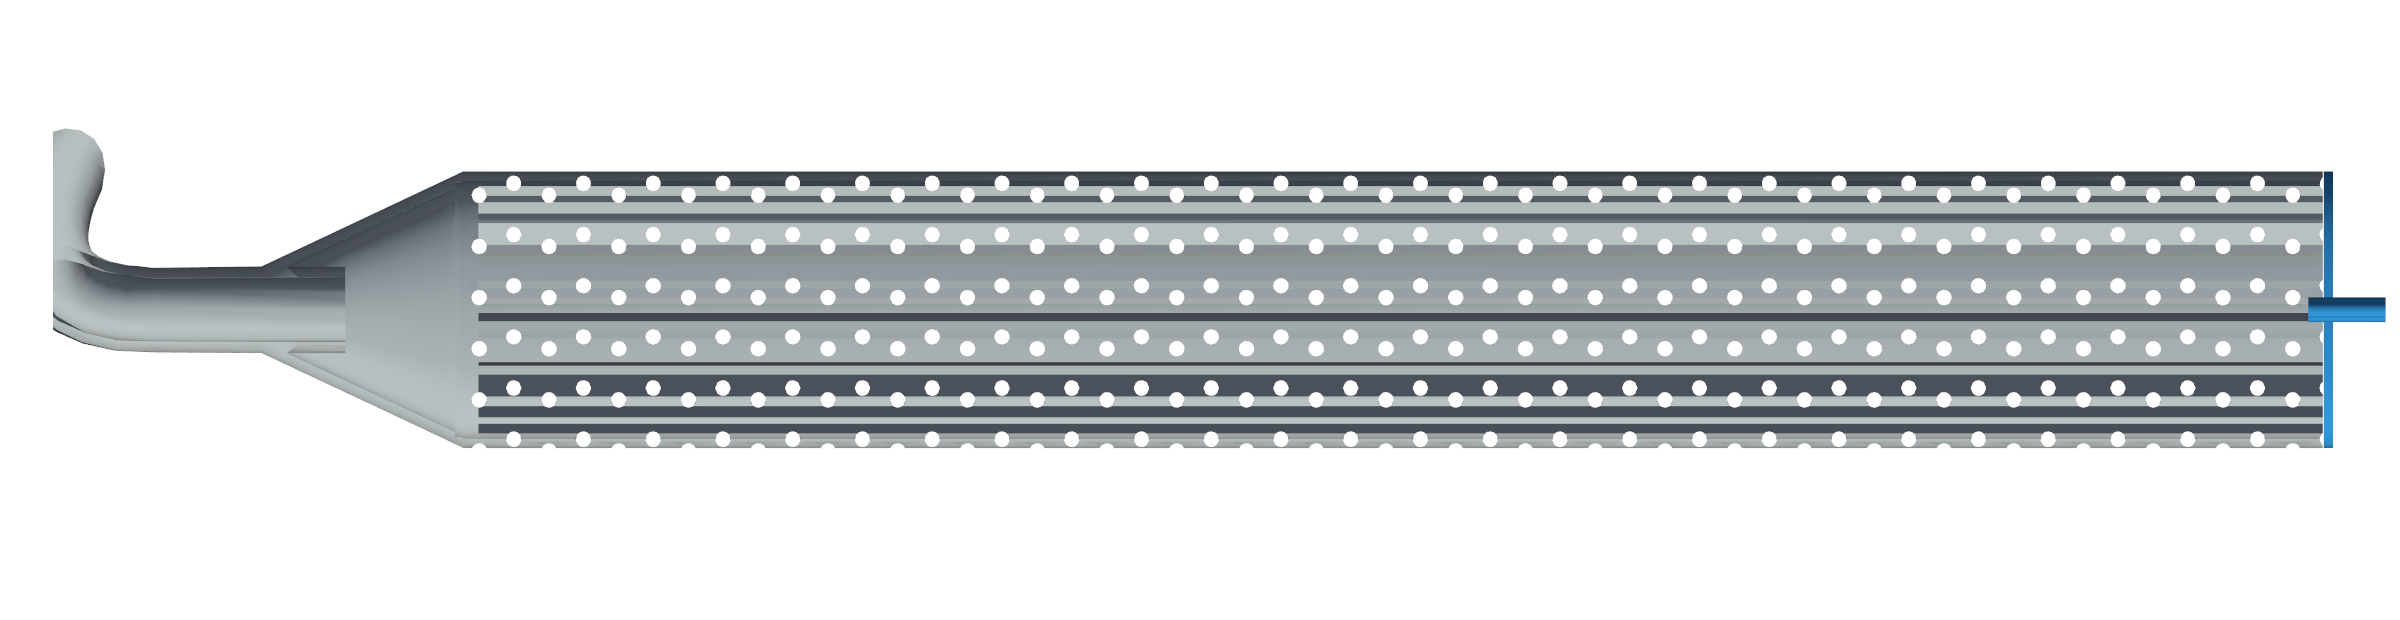
\includegraphics[width=0.95\linewidth]{fig_design.png}
\caption{The sheath cut open along its wide mid-plane. Suction tube and V-shaped funnel on the left, tip cap
with the irrigation outlet (blue) on the right. The internal tube is removed, all side holes are kept.}
\end{figure}
The sheath is \SI{120}{mm} long with an oval lumen of \SI{93.3}{mm^2} (\SI{11.1}{mL}). A funnel
\SI{7.6}{mm} long joins it to the suction tube (bore \SI{4.2}{mm}). The irrigation enters through a small
tube in the tip cap and points along the axis towards the suction.

\begin{center}\begin{tabular}{ll}\toprule
Fluid & water, $\rho=\SI{1000}{kg/m^3}$, $\mu=\SI{1}{mPa\,s}$, one phase only\\
Irrigation & \SI{250}{mL/h} $=\SI{4.17}{mL/min}$\\
Irrigation outlet & $d=\SI{1}{mm}$ (speed \SI{88}{mm/s}, $Re=88$); also $d=\SI{2}{mm}$ ($Re=44$)\\
Suction & $-\SI{7}{mmHg}=-\SI{933}{Pa}$ (the weakest of the range $-7$ to $-\SI{150}{mmHg}$)\\
Not modelled & air, tissue, wall deformation, clogging\\ \bottomrule
\end{tabular}\end{center}
All flows are laminar ($Re$ from 90 in the lumen jet to about 800 in the suction tube).

\section{Sheath blocked from outside}
With all holes blocked, only the irrigation flow itself can leave. The mean speed in the lumen is then
$U_m=Q/A=\SI{0.745}{mm/s}$, about 120 times slower than the jet. The jet drags fluid along; that fluid
cannot leave, so it returns along the walls as a ring vortex (figure~\ref{fig:field}).
\begin{figure}[h]\centering
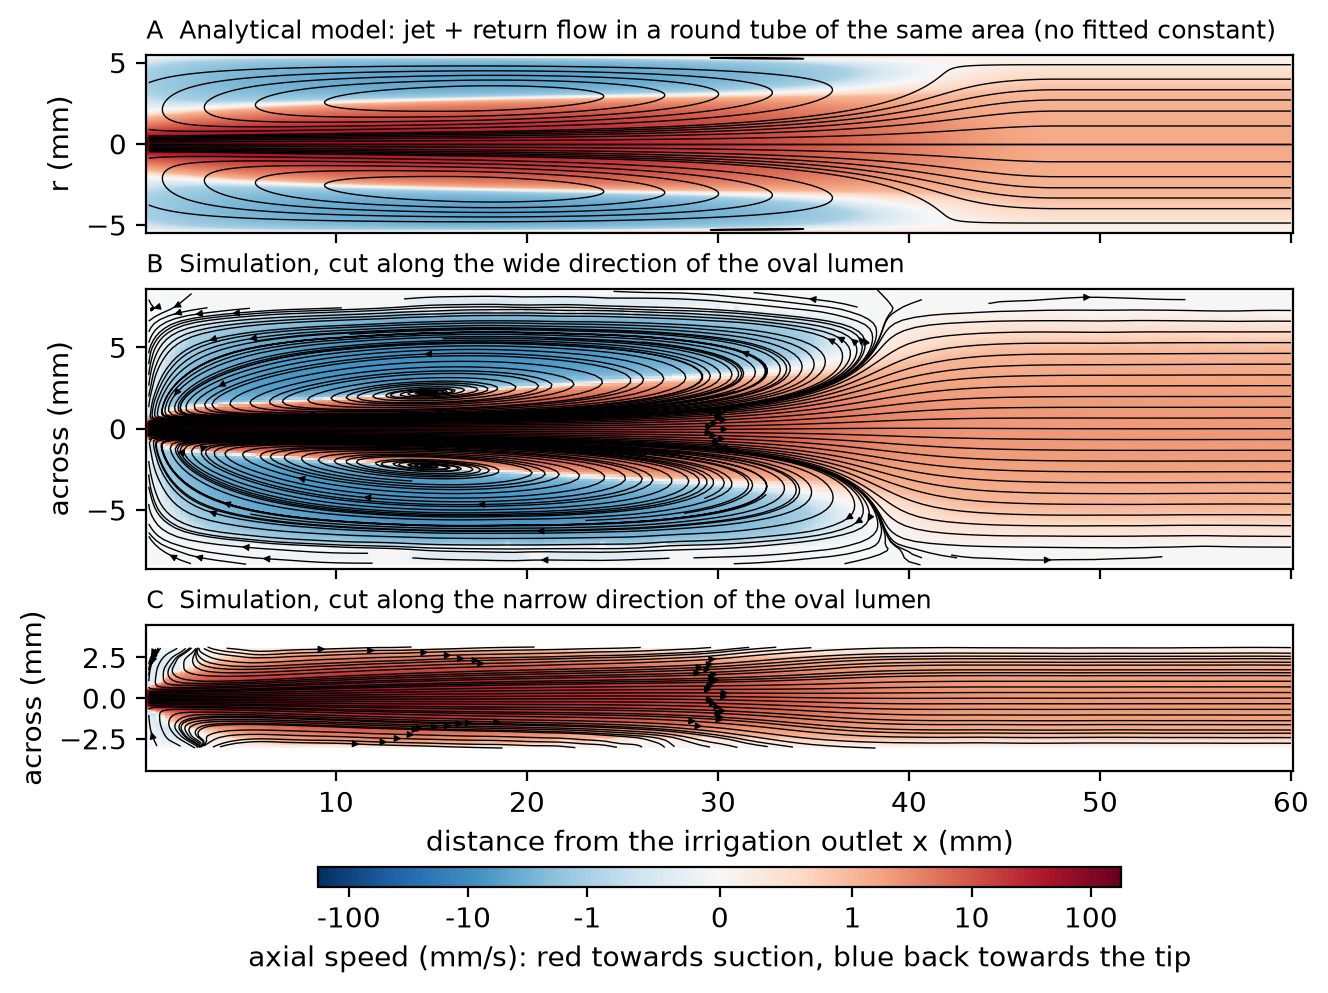
\includegraphics[width=0.86\linewidth]{fig_field.png}
\caption{Axial speed and streamlines near the outlet. A: analytical model. B, C: simulation, cut along the
wide and the narrow direction of the oval lumen.}\label{fig:field}
\end{figure}
\begin{center}\begin{tabular}{lrr}\toprule
 & Analytical & Simulation\\ \midrule
Build-up of return flow near the outlet (mL/min per mm) & 1.51 & 1.47\\
Peak return flow (mL/min) & 13.6 at \SI{17}{mm} & 10.1 at \SI{14}{mm}\\
Length of the vortex (mm) & 32 & 38\\
Centre speed far from the outlet (mm/s) & 1.5 (round tube) & 2.2\\
Pressure in the lumen (Pa) & $-933$, uniform & $-933$, uniform\\ \bottomrule
\end{tabular}\end{center}

\section{The mathematics in short}
The full derivation is in \texttt{jet\_loop\_maths.pdf}. The main steps:

\textbf{Jet.} The momentum flux of the jet, $K=\tfrac43U_j^2\,\pi d^2/4=\SI{8.19e-9}{m^4/s^2}$, is conserved.
The laminar round jet (Schlichting) then has centre speed and half-width
\begin{equation}
u_c(x)=\frac{3K}{8\pi\nu\,(x+x_0)},\qquad r_{1/2}=5.27\,\frac{\nu\,(x+x_0)}{\sqrt K},\qquad x_0=\frac{Re\,d}{16}=\SI{5.5}{mm},
\end{equation}
and takes in surrounding fluid at the rate $dQ/dx=8\pi\nu=\SI{1.51}{mL/min}$ per mm, whatever its momentum.

\textbf{Return flow.} The net flow through every cross-section is $Q$, so everything the jet takes in beyond
$Q$ must come back along the wall: $Q_{\rm back}(x)=Q_{\rm jet}(x)-Q$.

\textbf{End of the vortex.} The jet stops behaving as a jet when it fills the lumen
($r_{1/2}\approx 0.4\,R_{\rm eq}$, with $R_{\rm eq}=\sqrt{A/\pi}=\SI{5.45}{mm}$):
\begin{equation}
x_{\rm end}\approx Re\left(0.078\,R_{\rm eq}-\frac{d}{16}\right)
\quad\Rightarrow\quad \SI{32}{mm}\ (d=\SI{1}{mm}),\qquad \SI{13}{mm}\ (d=\SI{2}{mm}).\label{eq:xend}
\end{equation}
The vortex length is proportional to the irrigation rate and falls roughly as $1/d$.

\textbf{Open holes.} A hole of diameter $d_h$ under the pressure difference $\Delta p$ passes
$Q_h=C_d\,\tfrac{\pi}{4}d_h^2\sqrt{2\Delta p/\rho}$ with $C_d\approx0.61$, which gives the simulated
\SI{38}{mL/min} per hole.

\section{Sheath in fluid with some holes open}
Three cases were run with four open holes: near the tip, in the middle and near the connection.
\begin{center}\begin{tabular}{lrrr}\toprule
Open holes & Per hole, inwards (mL/min) & Suction (mL/min) & Irrigant out through holes\\ \midrule
near the tip & 37--39 & 154.7 & none\\
in the middle & 37--39 & 155.0 & none\\
near the connection & 37--38 & 155.1 & none\\ \bottomrule
\end{tabular}\end{center}
\begin{figure}[h]\centering
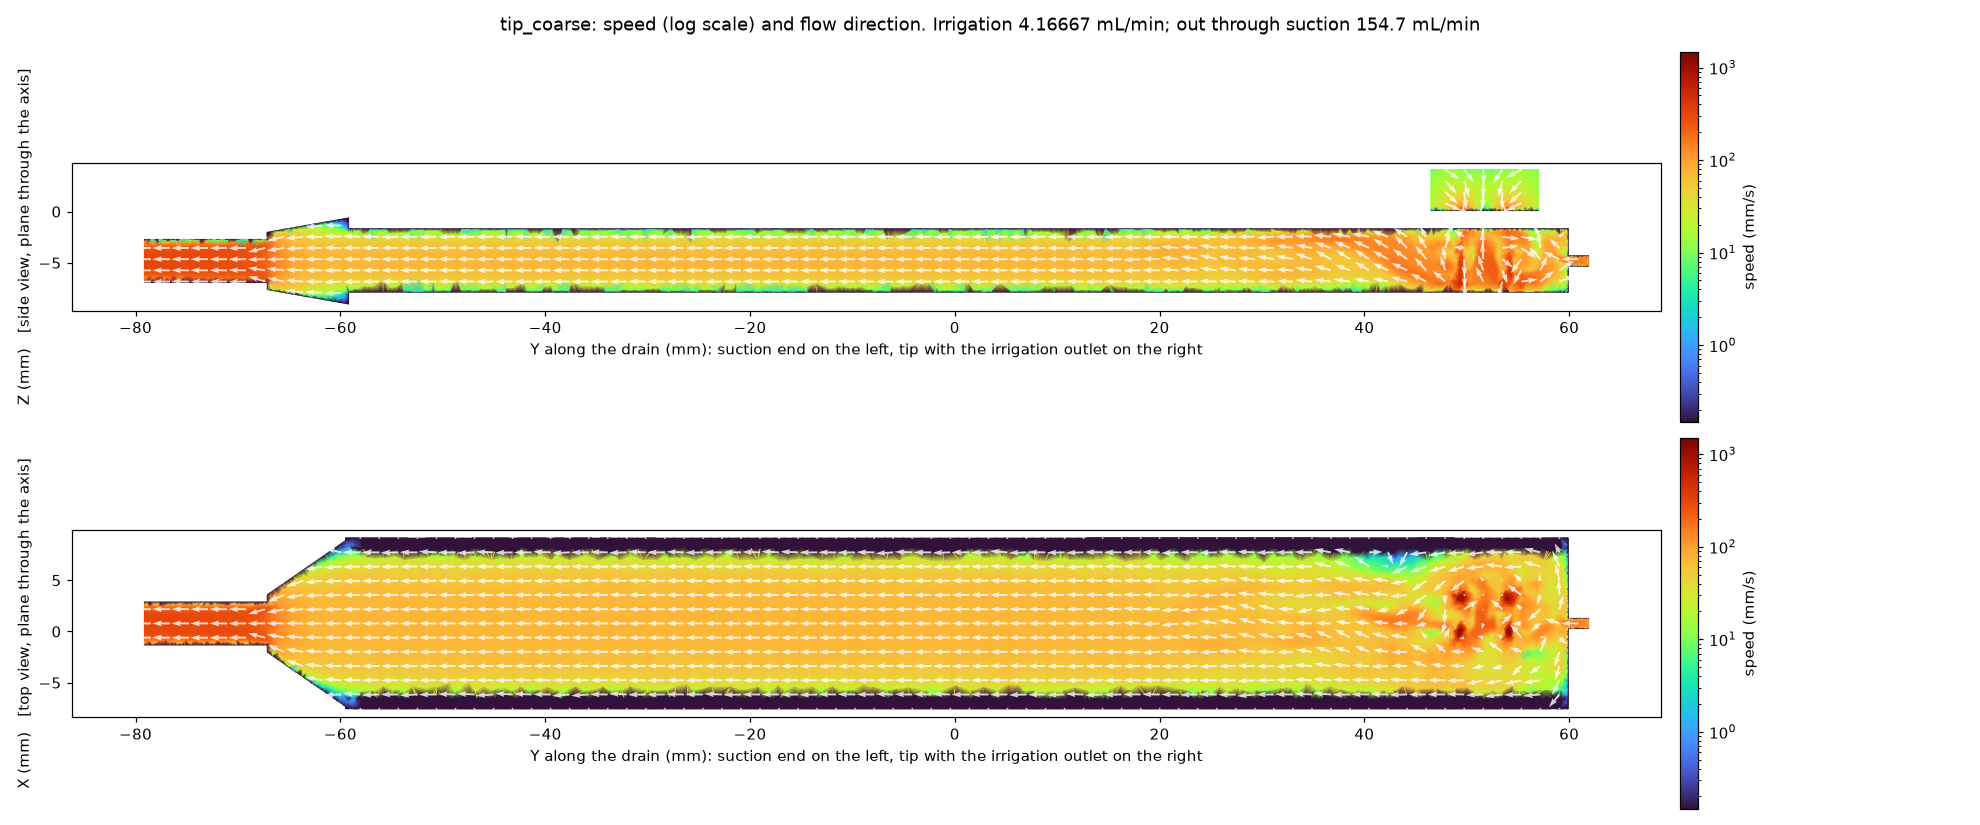
\includegraphics[width=0.95\linewidth]{tip_coarse/planes.png}
\caption{Four holes open near the tip: speed and flow direction on two planes through the axis. The hole
jets are far stronger than the irrigation jet.}
\end{figure}
The lumen is below bath pressure everywhere, so the holes can only draw in. These runs are short
(\SI{0.43}{s} of physical time on a coarse mesh) and the bath inflow is not fully balanced (22\,\%), so the
numbers are good to about that accuracy; the direction of the flow is not in doubt.

\section{Best position of the irrigation outlet}
\textbf{Method.} The outlet was moved from the tip to $s=15,30,45,60,80,\SI{100}{mm}$ from the tip, still
pointing at the suction, with all holes blocked (the worst case for flushing). For each position the steady
flow was computed. The lumen was then filled with 3000 markers of ``old fluid'', spread evenly over the
volume. Each marker is carried by the flow and also diffuses ($D=\SI{1e-9}{m^2/s}$, a small dissolved
molecule). A marker is counted as flushed when it reaches the suction tube. The score is the share of
markers still inside after a given time.
\begin{figure}[h]\centering
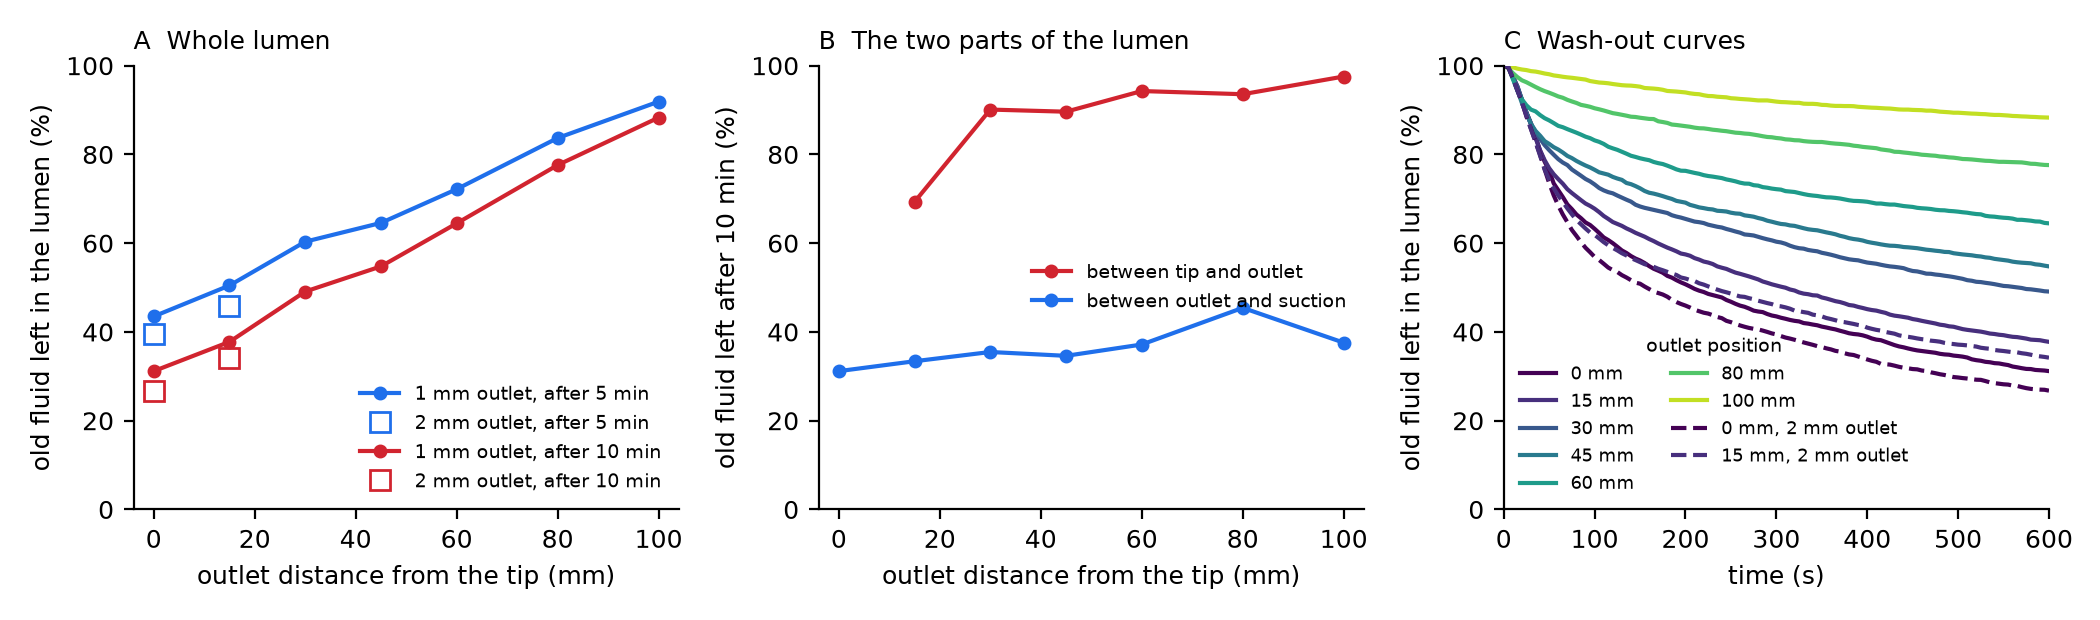
\includegraphics[width=\linewidth]{fig_sweep.png}
\caption{A: old fluid left in the whole lumen against outlet position. B: the same after \SI{10}{min},
separately for the part behind the outlet (tip side) and the part ahead of it (suction side). C: wash-out
curves.}\label{fig:sweep}
\end{figure}
\begin{center}\begin{tabular}{rrrrr}\toprule
Outlet from tip (mm) & Outlet $d$ (mm) & Left after 1 min & after 5 min & after 10 min\\ \midrule
0 (tip) & 1 & 72\,\% & 44\,\% & 31\,\%\\
15 & 1 & 74\,\% & 50\,\% & 38\,\%\\
30 & 1 & 79\,\% & 60\,\% & 49\,\%\\
45 & 1 & 81\,\% & 65\,\% & 55\,\%\\
60 & 1 & 86\,\% & 72\,\% & 64\,\%\\
80 & 1 & 93\,\% & 84\,\% & 78\,\%\\
100 & 1 & 98\,\% & 92\,\% & 88\,\%\\ \midrule
0 (tip) & 2 & 68\,\% & 39\,\% & 27\,\%\\
15 & 2 & 71\,\% & 46\,\% & 34\,\%\\ \bottomrule
\end{tabular}\end{center}
\begin{figure}[h]\centering
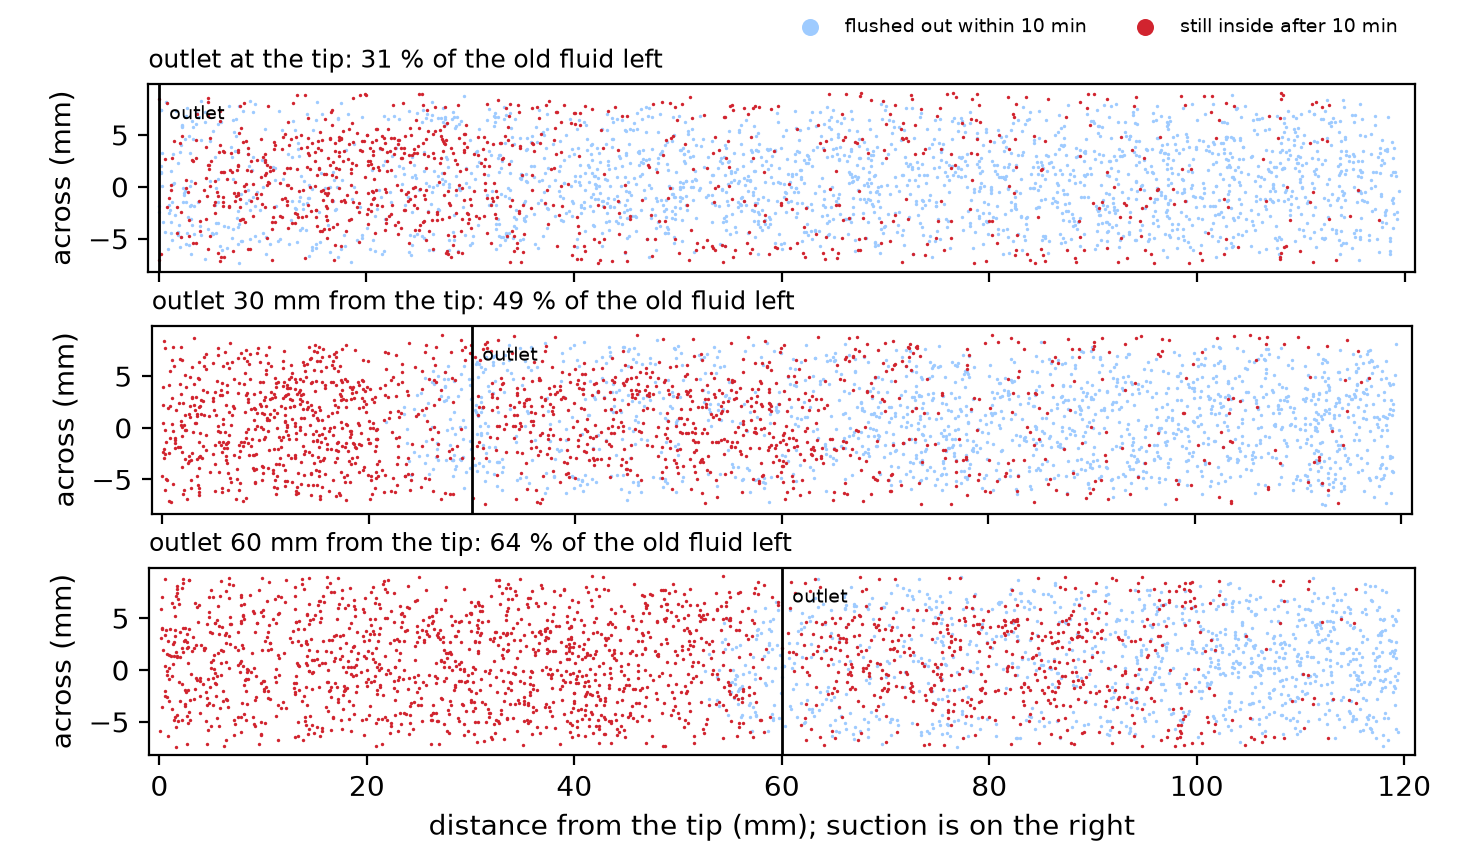
\includegraphics[width=0.92\linewidth]{fig_markers.png}
\caption{Where the old fluid that is still inside after \SI{10}{min} started (red), seen from the wide side.
Behind the outlet almost nothing is flushed. Just ahead of the outlet the ring vortex holds its fluid for
about \SI{40}{mm}. Further on, the slow duct flow carries the fluid out.}\label{fig:markers}
\end{figure}

\textbf{What the results say.}
\begin{itemize}\setlength\itemsep{1pt}
\item The score rises almost in a straight line with $s$. A simple rule reproduces it: with $L=\SI{119}{mm}$,
\begin{equation}
\phi(s)\approx\frac{s}{L}\,\phi_{\rm behind}+\Bigl(1-\frac{s}{L}\Bigr)\phi_{\rm ahead},\qquad
\phi_{\rm behind}\approx0.93,\quad \phi_{\rm ahead}\approx0.35\quad\text{(after \SI{10}{min})}.
\end{equation}
For $s=\SI{60}{mm}$ this gives 64\,\% (simulation 64\,\%), for $s=\SI{100}{mm}$ 84\,\% (simulation 88\,\%).
\item The fluid behind the outlet is a dead end. Only at $s=\SI{15}{mm}$ does the back of the vortex reach
part of it (69\,\% left instead of 90--98\,\%).
\item The vortex moves with the outlet (figure~\ref{fig:markers}). Wherever the outlet is, the next
\SI{40}{mm} are held by the vortex. Moving the outlet back does not remove this zone, it only adds dead
volume behind it.
\item The larger outlet helps a little, as eq.~\eqref{eq:xend} predicts: a shorter vortex traps less fluid.
\end{itemize}

\textbf{A correction.} The earlier version of the mathematics paper treated the vortex zone as a stirred tank
with a time constant of \SI{51}{s}. That is too optimistic. In steady laminar flow the streamlines of the
vortex are closed and fresh irrigation passes around it; without diffusion 86\,\% of the fluid that starts in
the vortex never leaves. The paper has been corrected.

\section{Recommendations}
\begin{enumerate}\setlength\itemsep{1pt}
\item Keep the irrigation outlet in the tip, pointing at the suction.
\item Prefer the larger outlet (\SI{2}{mm} rather than \SI{1}{mm}) at this flow rate: weaker jet, shorter
vortex, slightly better flushing.
\item Do not expect continuous irrigation alone to renew a fully blocked sheath quickly. Anything that
breaks the steady vortex should help: pulsed irrigation, a higher rate, or an open hole near the tip.
These were not simulated.
\end{enumerate}

\section{Limits}
\begin{itemize}\setlength\itemsep{1pt}
\item One fluid only: no air, tissue, clots or wall movement.
\item The position study used all holes blocked and suction at $-\SI{7}{mmHg}$ only. With holes open the
through-flow is about 40 times larger and the picture near the open holes changes.
\item The steady flows were stopped while still changing by about 0.2\,\% per step (the two \SI{2}{mm} runs
reached the steady-state tolerance). The score uses 3000 markers, so each value carries about
$\pm1$ percentage point of sampling noise. Both are small against the trend.
\item The marker step cannot cross walls and uses linear interpolation; fluid in the last cell layer at the
wall moves a little too slowly, which slightly overstates the fluid left in the grooves.
\item The flushing times depend on the diffusivity. $D=\SI{1e-9}{m^2/s}$ is right for small molecules; proteins
and cells diffuse 10 to 1000 times more slowly and would be held longer by the vortex.
\item The open-hole runs are short and on a coarse mesh (section 4).
\end{itemize}
\end{document}
